\documentclass[notes,11pt, aspectratio=169]{beamer}
\usetheme{default}
\usepackage{helvet}
\usepackage[default]{lato}
\usepackage{amsmath}
\usepackage{amsfonts}
\usepackage{amsthm}
\usepackage{mathpazo}
\usepackage{booktabs}
\usepackage{hyperref}
\usepackage{lipsum}
\usepackage{multimedia}
\usepackage{graphicx}
\usepackage{multirow}
\usepackage{graphicx}
\usepackage{changepage}
\usepackage{appendixnumberbeamer}
\newcommand{\beginbackup}{
   \newcounter{framenumbervorappendix}
   \setcounter{framenumbervorappendix}{\value{framenumber}}
   \setbeamertemplate{footline}
   {
     \leavevmode%
     \hline
     box{%
       \begin{beamercolorbox}[wd=\paperwidth,ht=2.25ex,dp=1ex,right]{footlinecolor}%
%         \insertframenumber  \hspace*{2ex}
       \end{beamercolorbox}}%
     \vskip0pt%
   }
 }
\newcommand{\backupend}{
   \addtocounter{framenumbervorappendix}{-\value{framenumber}}
   \addtocounter{framenumber}{\value{framenumbervorappendix}}
}
% These are my colors -- there are many like them, but these ones are mine.
\definecolor{blue}{RGB}{0,114,178}
\definecolor{red}{RGB}{213,94,0}
\definecolor{yellow}{RGB}{240,228,66}
\definecolor{green}{RGB}{0,158,115}

\hypersetup{
  colorlinks=false,
  linkbordercolor = {white},
  linkcolor = {blue}
}


%% I use a beige off white for my background
\definecolor{MyBackground}{RGB}{255,253,218}
\setbeamercolor{frametitle}{fg=blue}
\setbeamercolor{title}{fg=black}
\setbeamertemplate{footline}[frame number]
\setbeamertemplate{navigation symbols}{}
\setbeamertemplate{itemize items}{-}
\setbeamercolor{itemize item}{fg=blue}
\setbeamercolor{itemize subitem}{fg=blue}
\setbeamercolor{enumerate item}{fg=blue}
\setbeamercolor{enumerate subitem}{fg=blue}
\setbeamercolor{button}{bg=MyBackground,fg=blue,}
\setbeamercolor{section in toc}{fg=blue}
\setbeamercolor{subsection in toc}{fg=red}
\setbeamersize{text margin left=1em,text margin right=1em}

\newenvironment{wideitemize}{\itemize\addtolength{\itemsep}{0.4em}}{\enditemize}

% Customizing footer to display only the current page number
% Customizing footer: Right-aligned but with some padding from the edge
\setbeamertemplate{footline}{%
  \hfill
  \begin{beamercolorbox}[wd=\paperwidth,ht=0.4cm,dp=0.3cm,right]{footline}%
    \hspace{-1cm} \insertframenumber\hspace{0.2cm} % Adjust the spacing here
  \end{beamercolorbox}%
}

\title{\textcolor{blue}{Optimal public transportation networks:\\ \normalsize Evidence from the world's largest bus rapid transit system in Jakarta}}

\author{Gabriel Kreindler \and Arya Gaduh \and Tilman Graff \and Rema Hanna \and Benjamin A. Olken}

\institute{\textit{Conditionally accepted, AER}\\\vspace{1em} \large Presenter: Hyoungchul Kim}

\date{April 11, 2025}

\begin{document}

\begin{frame}[plain]
	\titlepage
\end{frame}

\setcounter{framenumber}{0}

\begin{frame}{Motivation: The challenges of public transport network design}
	\begin{wideitemize}
		\item Massive increase in private vehicles in LMICs.
			\begin{itemize}
				\item 10\% growth in private vehicles in India 2010-2019.
				\item Motorcycle ownership jumped from 37\% to 75.8\% in Jakarta 2002-2010. 
			\end{itemize}
		\item Large public transport investments and trend toward centralized operations.
			\begin{itemize}
				\item 100 LMIC cities with Bus Rapid Transit (BRT) in 2020, up from 14 in 2000.
			\end{itemize}
		\item This paper focuses on bus systems, which are important and flexible.
			\begin{itemize}
				\item India: 73\% urban public transport by bus (2011).
				\item Light infrastructure with low fixed cost of routes (unlike rail) $\Rightarrow$ Large design space.
			\end{itemize}
	\end{wideitemize}	
\end{frame}

\begin{frame}{Literature (skip)}
\begin{wideitemize}
\item Travel demand estimation, mode choice, and increasing returns in public transportation (McFadden 174; Ben-Akiva et al., 1985, Mohring, 1972).
\item Designing (road) transport network (Fajgelbaum and Schaal, 2020; Allenand Arkolakis, 2022; Balboni, 2021; Santamaria, 2022; Graff, 2024; Alder, 2023; Krantz, 2024).
\item Impact of transit systems in LMIC (Gaduh et al., 2022; Tsivanidis, 2024; Majid et al, 2018; Zarate, 2023; Balbonie t al, 2021).
\item Simulated annealing algorithm (Wei and Machemehl, 2006; Iliopoulou et al., 2019).
\end{wideitemize}	
\end{frame}

\begin{frame}{This paper\ldots}
	There are trade-offs in public transport network design. Based on how customers respond to changes in the design, we can estimate travel demand parameters relevant for optimal network design.

	\begin{table}
		\begin{center}
			\begin{tabular}{l|l}
			\toprule
			\textbf{Transport network design} & \textbf{Demand parameter}\\	
			\hline
			\textcolor{green}{Many lines vs. high frequency} & Value of wait time\\
			\hline
			\textcolor{green}{Direct lines vs. hub and spoke network} & Cost of transfers\\
			\hline
			\textcolor{green}{Dense converage vs. fast service} & Value of bus travel time\\
			\bottomrule
		\end{tabular}
	\end{center}
\end{table}\vspace{2em}

\textbf{This paper:} \textcolor{red}{Estimates these micro travel demand parameters relevant for optimal network design and show its implications on optimal network design.}
\end{frame}

\begin{frame}{Paper outline: Three steps}
	\begin{enumerate}
		\item Estimate the impact of Transjakarta's network expansion in 2016-2020 on ridership.
		\item use impact estimates and a demand model to infer how commuters value different dimensions of service quality: wait time, transfers, and bus travel time.
		\item Use estimates of the preference parameters to describe the shape of the optimal network.
	\end{enumerate}	\vspace{2em}

	\textbf{Warning:} Due to time constraint, some of the parts about the model will have to be more results-oriented.
\end{frame}

\begin{frame}{Institutional background}
	\textbf{The TransJakarta bus network}	
	\begin{wideitemize}
		\item Integrated bus system serving the central urban districts in Greater Jakarta (Daily ridership: 1 million in 2020).
		\item Over 139 bus route (BRT + Non-BRT), network length of more than 120 miles of BRT corridors.
		\item Primary public rapid transit system in the city (Primary alternative: private transport).
		\end{wideitemize}\vspace{1em}

	\textbf{TransJakarta bus network expansion}
	\begin{wideitemize}
	\item New 93 BRT and non-BRT routes (Jan 2016 - Feb 2020).
	\item \# of buses more than doubled (700 to 1600).
	\end{wideitemize}
\end{frame}

\begin{frame}{Expansion: Visualization}
	\begin{figure}
		\resizebox{0.7\textwidth}{!}{
		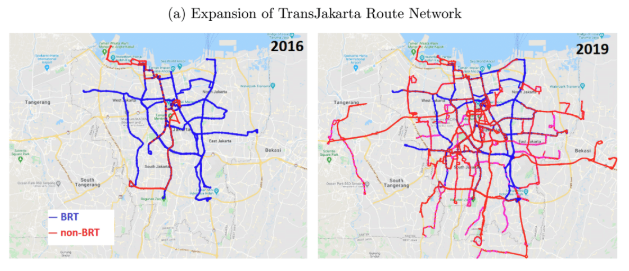
\includegraphics{expansion.png}
		}
	\end{figure}
\end{frame}

\begin{frame}{Data}

	\textbf{Geography}: Central urban districts divided into identical grid cells and aggregate stations at the grid cells level, and trips at the grid cell pair level.\vspace{1em}

	\textbf{Ridership data}
	\begin{wideitemize}
	\item Highly granular TransJakarta origin-destination ridership matrix at each point in time since 2016.
	\item Use algorithm to proxy rider's destination station.
	\end{wideitemize}\vspace{1em}

	\textbf{Aggregate trip flows}
	\begin{wideitemize}
	\item Smartphone data to construct aggregate trip flows (35 million trips, 2018 - 2020).
	\end{wideitemize}\vspace{1em}

	\textbf{Bus location and expansions}
	\begin{wideitemize}
	\item GPS location of buses and their routes to construct travel time, wait time, etc.
	\end{wideitemize}	
\end{frame}

\begin{frame}{Reduced-form: Impacts of expansion on ridership and on all trips}
	\textbf{3 variations induced by new route launch}
	\begin{wideitemize}
	\item \textcolor{red}{\textit{First direct route connection}} that is not faster than existing transfer (Event 1).
	\item \textcolor{red}{\textit{First direct route connection}} that is faster (Event 2).
	\item \textcolor{blue}{\textit{New route}} between two already connected: Arrival rate $\Uparrow$, wait time $\Downarrow$ (Event 3).
	\end{wideitemize}\vspace{1em}

	\textbf{Reduced-from specification (for each events)}
	\begin{align}
		\mathbb{E}Y_{odt} = \exp \left( \textcolor{red}{\alpha} Post_{odt} + \alpha_{-10} L_{\leq -10, odt} + \alpha_{10}L_{\geq 10,odt} + \mu_{od} + \nu_{ot} + \xi_{dt} + \varepsilon_{odt} \right) 		\nonumber
	\end{align}\vspace{-1em}
	\begin{itemize}
		\item $Post_{odt}$: Indicator variable for the event having taken place on the $(o,d)$ route in the previous 10 months.
		\item $L_{\leq -10, odt}, L_{\geq 10,odt}$: Indicators for whether an event between o and d takes place 10 or more months in the future, and in the past, respectively. 
	\end{itemize}
\end{frame}

\begin{frame}{Results: Impacts on ridership}
	\begin{columns}
	\begin{column}{0.7\textwidth}
	\begin{figure}
		\resizebox{0.9\textwidth}{!}{
		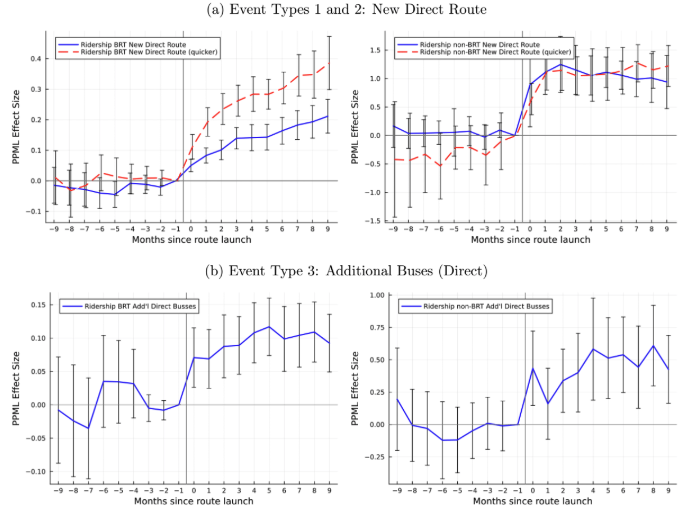
\includegraphics{ridership.png}
		}
	\end{figure}
\end{column}
\begin{column}{0.3\textwidth}
\begin{wideitemize}
\item \textbf{Event 1}: $\sim 15.9\%$ (BRT) ridership increase.
\item \textbf{Event 2}: $\sim 20.7\%$ (BRT) ridership increase.
\item \textbf{Event 3}: $\sim 9.6\%$ (BRT) $\sim 56.8\%$ (non-BRT)  ridership increase.
\end{wideitemize}	
\end{column}
\end{columns}
\end{frame}

\begin{frame}{Results: Impacts on aggregate trip volume}
	\begin{figure}
		\resizebox{0.7\textwidth}{!}{
		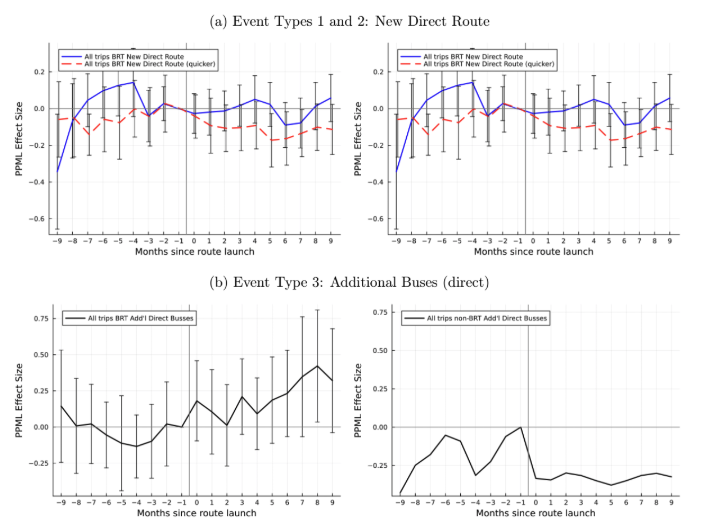
\includegraphics{agg-trip.png}
		}
	\end{figure}
\end{frame}

\begin{frame}
	\centering
	\Huge{Model}
\end{frame}

\begin{frame}{Modeling travel demand}
\begin{wideitemize}
\item Develop a travel demand model and estimate the \textcolor{blue}{set of riders' preferences parameters that best match the reduced-form estimates.}
	\item Nested travel demand model:	
	\begin{enumerate}
		\item \textbf{Outer nest}: Commuter chooses between bus vs. outside private mode.
		\item \textbf{Inner nest}: Then commuter chooses preferred bus route within the TransJakarta network. 
	\end{enumerate}	
\item In the model, a commuter's utility is given by:
	\begin{itemize}
		\item \textcolor{blue}{travel time} on the bus.
		\item \textcolor{blue}{bus transfer cost}.
		\item bus \textcolor{blue}{wait time}.
		\item esimated with $o-d$ fixed effects and an \textcolor{blue}{inattention} parameter.
	\end{itemize}
\end{wideitemize}



\end{frame}

\begin{frame}{Model setup: Bus route choice model (brief)}
	\textbf{Basic setup}: Static discrete choice model (over bus options) with idiosyncratic heterogeneity from exponentially distributed random wait times.	
	\begin{wideitemize}
	\item Commuter $i$ chooses travel option that maximize his utility of going from $o$ to $d$.
	\item Random utility component comes from wait time (Poisson process).
	\item[] $u_k = \underbrace{-\alpha_{time}T_k^{time}}_{\hidewidth v_k \hidewidth} - \alpha_{wait} \omega_k$, $\omega_k$ (wait time) is drawn from exponential distribution.
	\item If commuters choose transfer option:\\
	$u_k = \alpha_{time} T_{k1}^{time} + \mathbb{E}\max_{k2} \left[ -\alpha_{time} T_{k2}^{time} - \alpha_{wait} T_{k2}^{wait} \right] + \mu_{transfer} - \alpha_{wait} T_{k1}^{wait}.$
\item In higher decision nest: Commuter decide whether to use TransJarkarta network or alternative ($u_{it}^{bus}$ vs. $u_{it}^{private}$).
	\end{wideitemize}
\end{frame}

\begin{frame}{Model estimation (brief)}
	\textbf{Parameters to estimate}: $\theta = \left( \sigma, \alpha_{wait}^{BRT}, \mu_{transfer}^{BRT}, \eta^{BRT}, \alpha_{wait}^{non-BRT}, \mu_{transfer}^{non-BRT}, \eta^{non-BTR} \right)\vspace{1em}

	\begin{block}{Esimation approach (very brief)}
		\begin{wideitemize}
		\item Match reduced-form event study coefficients with the model.
		\item Apply classical minimum distance estimation to retrieve parameters: 
		\item[] $\min_{\theta} (\underbrace{m(\theta)}_{\hidewidth \text{model moments} \hidewidth} - \overbrace{\widehat{m}}^{\hidewidth \text{empirical estimates} \hidewidth})' \widehat{W} (m(\theta) - \widehat{m})$
		\end{wideitemize}	
	\end{block}
\end{frame}

\begin{frame}{Esimation results}
	\begin{columns}
		\begin{column}{0.5\textwidth}
	\begin{figure}
		\resizebox{\textwidth}{!}{
			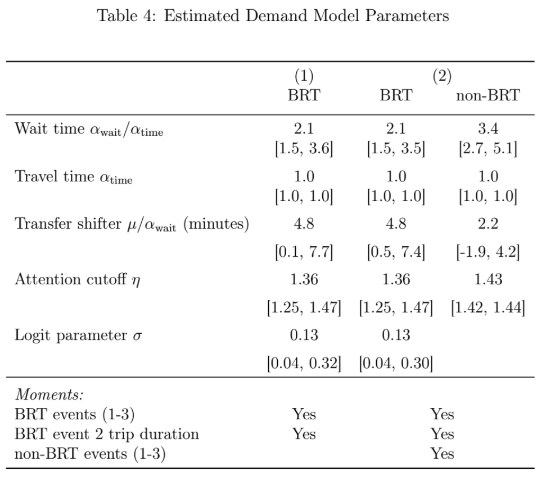
\includegraphics{demand-par.png}
		}
	\end{figure}
\end{column}
\begin{column}{0.5\textwidth}
\begin{wideitemize}
\item Travelers dislike wait time 2.1x (BRT) and 3.4x (non-BRT) more than travel time on the bus.
\item Close to zero transfer penalty: Dislike of bus transfer is lower?
\item Travelers tend to not consider bus options with travel time 36\% (BRT) and 43\% (non-BRT) slower than quickest option.
\end{wideitemize}	
\end{column}
\end{columns}
\end{frame}

\begin{frame}{Intuitions for network design}
	\textbf{Geography}
	\begin{wideitemize}
	\item $418$ $2\times 2$ km square grid cells, leading to 1,536 adjacency links (potential bus route path).
	\item Bus travel time calculated for each grid edge.
	\end{wideitemize}\vspace{1em}

	\textbf{Environment}
	\begin{wideitemize}
	\item Network $N$: Set of routes with bus allocations (1,500 buses in total).	
	\item Model welfare $W(N, \theta)$.
	\item Estimated preferences parameter $\theta$.
	\end{wideitemize}\vspace{0.5em}

	\begin{block}{\centering \textbf{Objective}}
		\centering
		Optimal network $N^*$ that maximizes welfare.	
	\end{block}
\end{frame}

\begin{frame}{Current vs. optimal network design}
	\begin{columns}
	\begin{column}{0.6\textwidth}
	\begin{figure}
		\resizebox{\textwidth}{!}{
		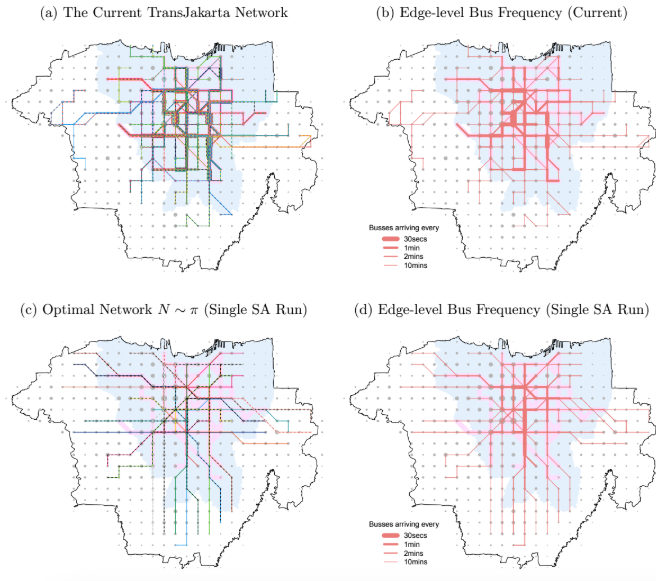
\includegraphics{optimal-fig.png}
		}
	\end{figure}
\end{column}
\begin{column}{0.4\textwidth}
	\begin{wideitemize}
	\item \textbf{Current}: Buses concentrated in the city center (short wait time in center, long wait time in outer part).
	\item \textbf{Optimal}: A more expansive network (spread out).
	\item Caveat: Not considering constraints preventing the expansion.
	\end{wideitemize}	
\end{column}
\end{columns}
\end{frame}

\begin{frame}{Conclusion}
	\begin{wideitemize}
		\item Additional direct route option leads to increase in ridership.
		\item Commuter are responsive to public transport (non-price) service improvements (wait-time, travel-time, etc).
		\item Optimal network suggests that more expansive network could increase commuters' welfare and ridership. 
		\item Kudos to them for conditional accept at AER!
	\end{wideitemize}	
\end{frame}

\end{document}
